\section{理想反应器的停留时间分布}


\begin{frame}
    \frametitle{活塞流模型}

    活塞流模型的停留时间特征就是同时进入系统的流体粒子也同时离开系统。

    若在$t=0$时向活塞流反应器的进口以$\delta$函数的形式脉冲输入示踪剂时，则其出口流体中示踪剂的浓度也呈$\delta$函数的形式。

    \begin{minipage}{0.38\linewidth}
        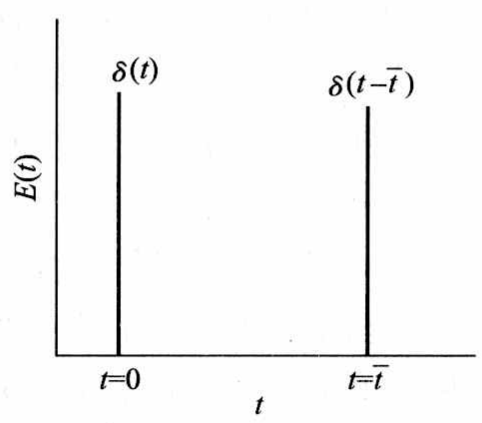
\includegraphics[width=\linewidth]{figures/fig5.7.png}
    \end{minipage}\hfill
    \begin{minipage}{0.58\linewidth}
        \[
            E(t) = \delta (t- \bar t)
        \]
        \[
            E(\theta ) = \delta (\theta- 1)
        \]
        \[
            \bar{\theta}=\int_{0}^{\infty} \theta \delta(\theta-1) \mathrm{d} \theta=\theta|_{1}=1 
        \]
        \[
            \sigma_{\theta}^{2}=\int_{0}^{\infty} \theta^{2} \delta(\theta-1) \mathrm{d} \theta-1=\theta^{2}|_{1}-1=0
        \]
    \end{minipage}

\end{frame}


\begin{frame}
    \frametitle{活塞流模型}

    \begin{minipage}{0.54\linewidth}
        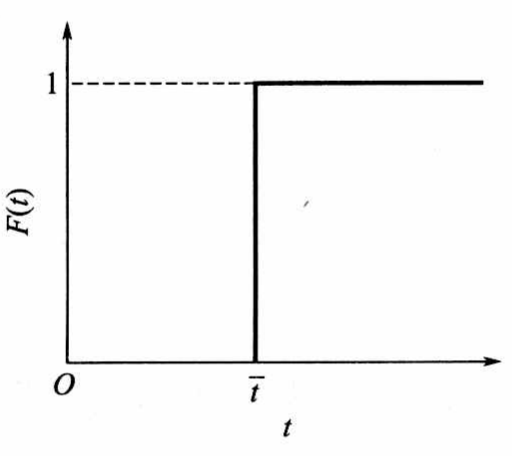
\includegraphics[width=\linewidth]{figures/fig5.8.png}
    \end{minipage}\hfill
    \begin{minipage}{0.44\linewidth}
        $F(t)=\left\{\begin{array}{ll}
            0 \quad \quad & t<\bar{t} \\
            1 \quad \quad & t \geqslant \bar{t}
            \end{array}\right.$

        \bigskip

        $F(\theta)=\left\{\begin{array}{ll}
            0 \quad \quad & \theta<1 \\
            1 \quad \quad & \theta \geqslant 1
            \end{array}\right.$
    \end{minipage}

\end{frame}


\begin{frame}
    \frametitle{全混流模型}

    设连续进入全混流反应器的流体中示踪剂的浓度为$c_0$，则单位时间内流入反应器及从反应器流出的示踪剂量分别为$Qc_0$和$Qc$。由于反应器内示踪剂的浓度均一且等于出口流中的示踪剂浓度，所以，单位时间内反应器内示踪剂的累积量为$V_r \dif c/ \dif t$，于是对反应器作示踪剂的物料衡算得
    \[
        V_r \frac{\dif c}{\dif t} = Qc_0 - Qc
    \]
    将$\tau =V_r/Q_0$代入，得
    \[
        \frac{\dif c}{\dif t} + \frac{1}{\tau}c = \frac{1}{\tau}c_0
    \]
    积分得
    \[
        \ln \frac{c_0 - c}{c_0} = - \frac{t}{\tau} \qquad \text{或} \qquad 1- \frac{c}{c_0} = e^{-t/\tau}
    \]

\end{frame}


\begin{frame}
    \frametitle{全混流模型}
    
    根据$F(t)=\frac{c(t)}{c(\infty)}=\frac{c(t)}{c(0)}$得
    \[
        F(t) = 1 - e^{-t/\tau}
    \]
    对$t$求导，得
    \[
        E(t) = \frac{1}{\tau}e^{-t/\tau}
    \]
    若采用无因次时间，则
    \[
        F(\theta) = 1 - e^{-\theta}
    \]
    对$t$求导，得
    \[
        E(\theta) = e^{-\theta}
    \]
    全混流反应器的$\bar \theta = 1$，方差$\sigma _ \theta ^2 =1$，返混程度最大。

\end{frame}


\begin{frame}
    \frametitle{全混流模型}

    \begin{figure}
        \centering
        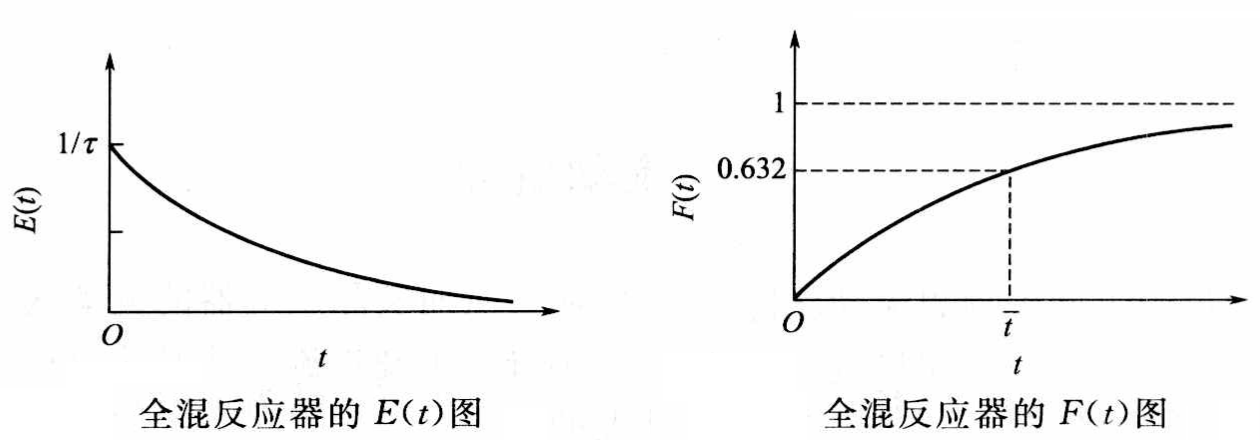
\includegraphics[width=\linewidth]{figures/fig5.9.png}
    \end{figure}
    全混流反应器，停留时间小于平均停留时间的流体粒子占全部流体的分率为$F(\bar t)=1-e^{-1}=0.632$，这部分流体的转化率小于活塞流反应器是毫无疑义的。
\end{frame}


\begin{frame}
    \frametitle{全混流模型的平均停留时间和方差}
    \[
        \begin{aligned}
            \bar{\theta}&=\int_{0}^{\infty} \theta E(\theta) \mathrm{d} \theta \\
            & = \int_{0}^{\infty} \theta e^{-\theta} \mathrm{d} \theta \\
            & = 1 \\
            \sigma_{\theta}^{2}&=\int_{0}^{\infty} \theta^{2} E(\theta) \mathrm{d} \theta-1 \\
            & = \int_{0}^{\infty} \theta^{2} e^{-\theta} \mathrm{d} \theta-1 \\
            & = 1
        \end{aligned}
    \]
\end{frame}


\begin{frame}[t]
    \frametitle{}

    \begin{example}
        设$F(\theta)$及$E(\theta)$分别为闭式流动反应器的停留时间分布函数及停留时间分布密度。

        若该反应器为活塞流反应器，下列值是多少？若该反应器为全混流反应器，下列值是多少？

        $F(1); \quad E(1); \quad F(0.8); \quad E(0.8); \quad E(1.2)$        

    \end{example}

\end{frame}